\section{Respuesta en frecuencia}

Se estudiará la ganancia del circuito y la diferencia de fase entre la señal de entrada y salida en respuesta a la frecuencia con los dos circuitos propuestos. Se iniciará con la construcción de los modelos teóricos para seguidamente compararlos con los datos recogidos de las mediciones y simulaciones.  

Durante el análisis, es importante tener en cuenta parámetros del amplificador operacional tal como su ganancia a lazo abierto, $A_{ol}$, y su Producto de Ancho de Banda (Gain–bandwidth product, GBW). Éste último resulta de especial interés al momento de diseñar un circuito que contenga un $Op Amp$. El GBW del operacional es igual al producto entre la ganancia a alzo abierto y el ancho de banda del circuito, y especifica la frecuencia alrededor de la cual el operacional, sin retroalimentación, deja de amplificar la señal de entrada. Es decir, es importante elegir un amplificador operacional que trabaje de la manera deseada para el rango de frecuencias a la cual operará el circuito.  

\subsection{Circuito inversor}

\subsubsection{Análisis teórico}

Partiendo de condiciones ideales de un amplificador operacional, tales como corriente de entrada a los terminales y tensión de offset nulas,
impedancia de entrada infinita e impedancia de salida igual a cero, la tensión de salida del dispositivo esta dado por el producto de la tensión de entrada diferencial
y la ganancia a lazo abierto del amplificador (sin retroalimentación), donde para el circuito inversor de la Figura resulta:

\begin{equation} \label{eq:1}
	v_{out}=A_{v}v_{d}=A_{v_{ol}}(v^{+}-v^{-})=-A_{v_{ol}}v^{-}
\end{equation}

Se plantean las siguientes ecuaciones que describen al circuito inversor de la Figura:

\begin{equation}
\left\{\begin{matrix}

	$$I_{3}=-\frac{v^{-}}{R_{3}}$$
	
	\\ 
	$$I_{1}=\frac{v_{in}-v^{-}}{R_{1}}$$
	
	\\ 
	
	$$I_{2}=\frac{v^{-}-V_{out}}{R_{2}}$$
	
	\\ 
	
	$$I_{1}=I_{2}+I_{3}$$
	
	\end{matrix}\right.
\end{equation}
Resolviendo el sistema con la relación \ref{eq:1} se obtiene que:

\begin{equation} 
	\frac{v_{out}}{v_{in}}=-\frac{A_{v_{ol}}\frac{R_{2}}{R_{1}}}{A_{v_{ol}}+\frac{R_{1}R_{3}+R_{1}R_{2}+R_{2}R_{3}}{R_{1}R_{3}}}
    k=\frac{R_{1}R_{3}+R_{1}R_{2}+R_{2}R_{3}}{R_{1}R_{3}}
\end{equation}

De modo que la función transferencia resulta:

$$H(s)=\frac{-\frac{R_{2}}{R_{1}}}{1+\frac{k}{A_{v_{ol}}}}$$

Si se considera a la ganancia de tensión como infinita, se obtiene:

$$A_{v_{ol}}\underset{\infty }{\rightarrow} \frac{v_{out}}{v_{in}}=-\frac{R_{2}}{R_{1}}=G_{ideal}$$

Correspondiendo con lo estudiado en el curso para circuitos inversores. 

En el caso que la ganancia de tensión del operacional sea un valor constante, se tiene:

$$A_{v_{ol}}=A_{ol}\Rightarrow H(s)=\frac{G_{ideal}}{1+\frac{k}{A_{ol}}}$$

Considerando el modelo de compensación de polo dominante, se expresa la ganancia a lazo abierto (ganancia sin retroalimentación) como una función
de primer orden dada por:

$$A_{v} = \frac{A_{ol}}{1+\frac{s}{w_{b}}}$$

Donde $A_{ol}$ es la ganancia a lazo abierto y $w_{b}$ es el ancho de banda del operacional, ambos parámetros propios del amplificador. 
Reemplazando en la función de transferencia y tomando que $\frac{k}{A_{ol}}\approx 0$ para los casos estudiados, resulta:

$$A_{v} = \frac{A_{ol}}{1+\frac{s}{w_{b}}}\Rightarrow H(s)=\frac{G_{ideal}}{1+\frac{k}{A_{ol}}+\frac{s}{w_{b'}}}$$

$$w_{b'} = \frac{A_{ol}w_{b}}{k}$$

Teniendo en cuenta que $GBW = w_{b}A_{ol}$, reemplazando los valores en las funciones descriptas se obtienen las siguientes expresiones considerando cada caso del circuito inversor:

\begin{table}[H]
\centering
\begin{tabular}{c|c|c|c}
       & $A_{ol} = \infty$  & $A_{ol} = 10^{5}$ & $A_{v} = \frac{A_{ol}}{1+\frac{s}{w_{b}}}$ \\ \hline
Caso 1 & -10  & $-9.998$  & $H(s)=\frac{-10}{17,5\cdot 10^{-6}+1}$  \\ \cline{1-1}
Caso 2 & -1  & $-0.999$   & $H(s)=\frac{-1}{2,5\cdot 10^{-6}+1}$  \\ \cline{1-1}
Caso 3 & -0.1  & $-0.099$  & $H(s)=\frac{-0.1}{1\cdot 10^{-6}+1}$

\end{tabular}
\end{table}

\begin{figure}[H]
	\begin{subfigure}{1\textwidth}
	    \centering
		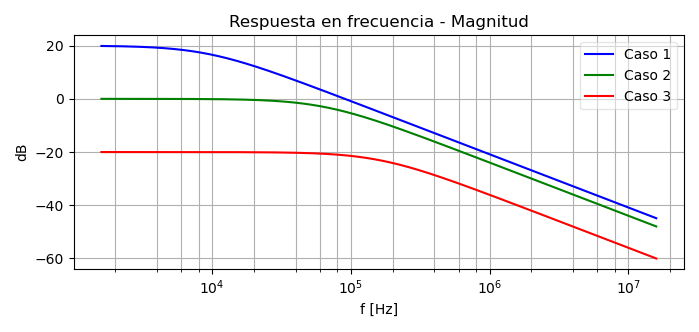
\includegraphics[width=.8\linewidth]{./Imagenes/InversorCasosGain.png}  
		\caption{Respuesta en frecuencia teórica: ganancia}
	\end{subfigure}
	\newline
	\begin{subfigure}{1\textwidth}
	    \centering
		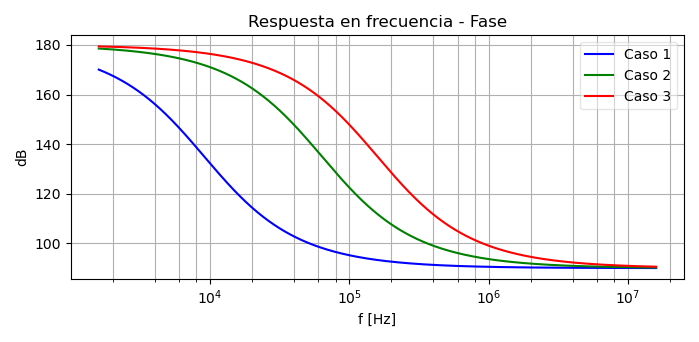
\includegraphics[width=.8\linewidth]{./Imagenes/InversorCasosPhase.png}  
		\caption{Respuesta en frecuencia teórica: fase}
	\end{subfigure}
	\caption{Circuito inversor. Respuesta en frecuencia teórica.}
	\label{fig:invcasos}
\end{figure} 

En la figura \ref{fig:invcasos} se graficaron conjuntamente los tres casos de la configuración inversora considerando el modelo de polo dominante. Se puede visualizar que 
a muy bajas frecuencias las ganancias se corresponden con los casos mas ideales ($A_{v_{ol}}$ infinito o constante), aproximando la ganancia a la relación entre $R_{1}$ y $R_{2}$. Se observa, además, que la diferencia de fase entre la señal de entrada y la de salida a bajas frecuencias es de alrededor de $180^{\circ}$, lo cual es correcto considerando que el circuito actúa como inversor. 
Asimismo, se puede observar que el Caso 3 presenta la frecuencia de corte mas elevada. 

\subsubsection{Resultados}

Se realizaron los circuitos utilizando el $Digilent$ $Electronics$ $Explorer$, mediante el cual se tomaron mediciones de la tensión de entrada, de salida y la fase entre ambas en el rango de frecuencias
consideradas de interés en cada caso, de modo de obtener un gráfico de su ganancia y cambio de fase en respuesta a la frecuencia. Para la medición de los mismos, en cada caso se intentó prever los efectos del 
Slew Rate empleando una tensión de entrada que no se vea afectada por el mismo. Por otro lado, se simularon los circuitos en LTSpice. 

Para el armado del circuito, se utilizó un operacional de los cuatro presentes en el integrado, conectando en el resto sus entradas no inversoras a GND y las entradas inversoras con su respectiva salida.
Se intentó evitar el uso de cables entre los componentes para minimizar al máximo las pérdidas. Se presenta una foto de la configuración inversora utilizada para las mediciones de la ganancia y diferencia de fase 
en respuesta a la frecuencia.

\begin{figure}[H]
	\centering
	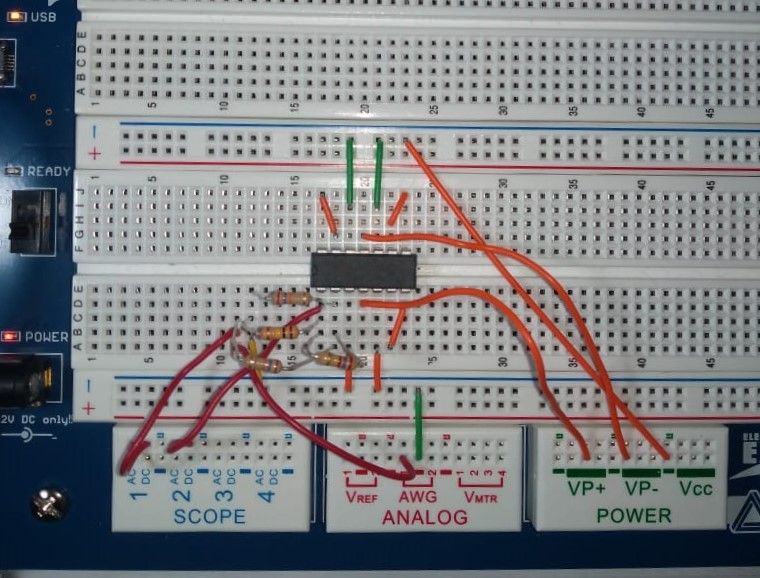
\includegraphics[scale=0.5]{./Imagenes/Inv3Freq.jpeg}
	\caption{Circuito inversor Caso 3 en el Digilent Electronics Explorer}
	\label{fig:circinvcaso1}
\end{figure}

\begin{figure}[H]
	\centering
	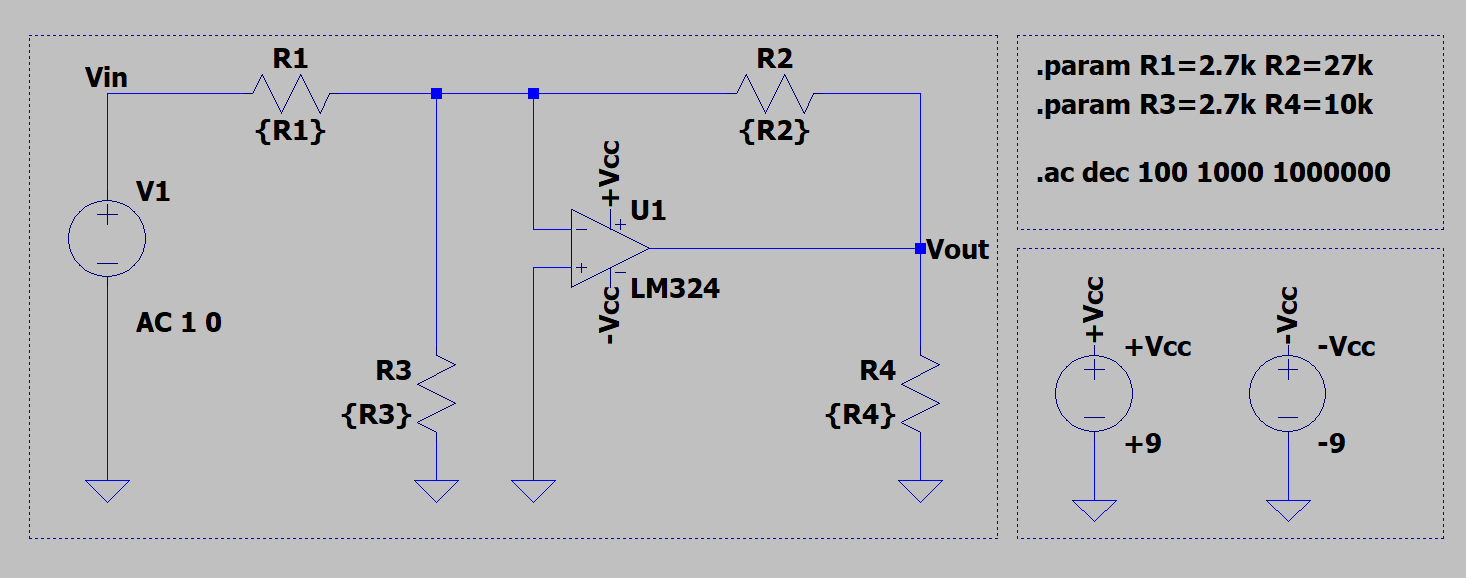
\includegraphics[scale=0.35]{./Imagenes/simuInv1.png}
	\caption{Esquema circuital inversor Caso 1 en LTSpice}
	\label{fig:circinvcaso1}
\end{figure}

Se superpusieron los resultados con la función transferencia teórica, obteniendo los siguientes resultados:

\begin{figure}[H]
	\centering
		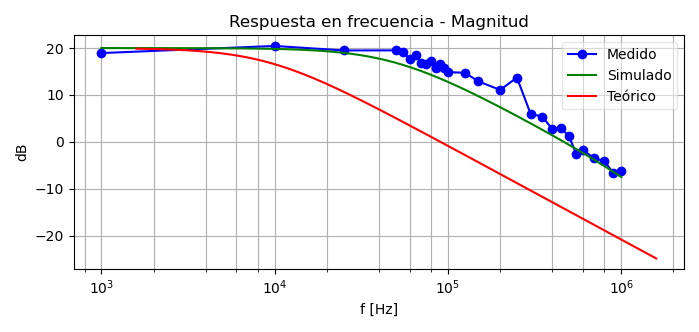
\includegraphics[width=.8\linewidth]{./Imagenes/InvCaso1Gain.png}  
		\caption{Inversor Caso 1. Respuesta en frecuencia teórica: ganancia}
	\label{fig:circinvcaso1}
\end{figure}

\begin{figure}[H]
	\centering
		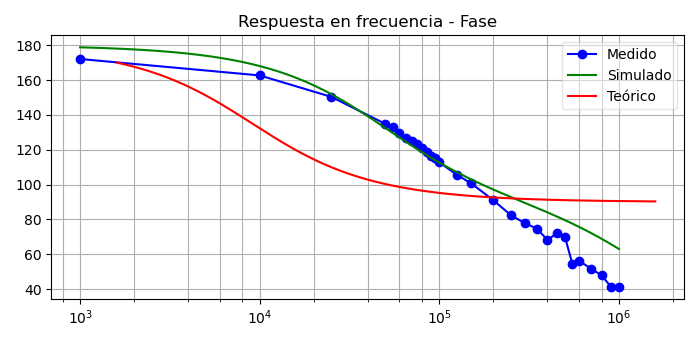
\includegraphics[width=.8\linewidth]{./Imagenes/InvCaso1Phase.png}  
		\caption{Inversor Caso 1. Respuesta en frecuencia teórica: fase}
	\label{fig:circinvcaso1}
\end{figure}

\begin{figure}[H]
	\centering
		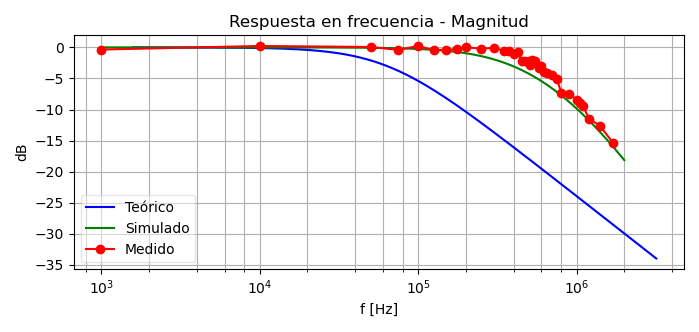
\includegraphics[width=.8\linewidth]{./Imagenes/InvCaso2Gain.png}  
		\caption{Inversor Caso 2. Respuesta en frecuencia teórica: ganancia}
	\label{fig:circinvcaso1}
\end{figure}

\begin{figure}[H]
	\centering
		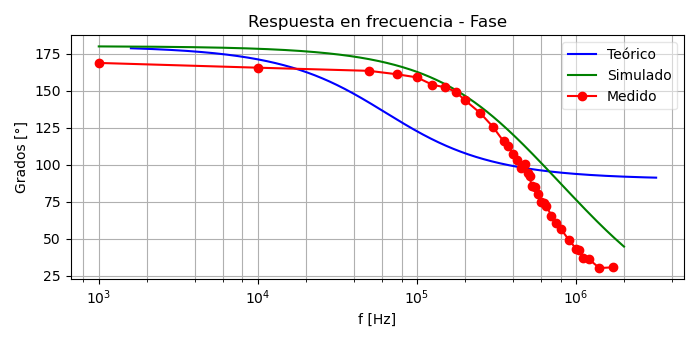
\includegraphics[width=.8\linewidth]{./Imagenes/InvCaso2Phase.png}  
		\caption{Inversor Caso 2. Respuesta en frecuencia teórica: fase}
	\label{fig:circinvcaso1}
\end{figure}

\begin{figure}[H]
	\centering
		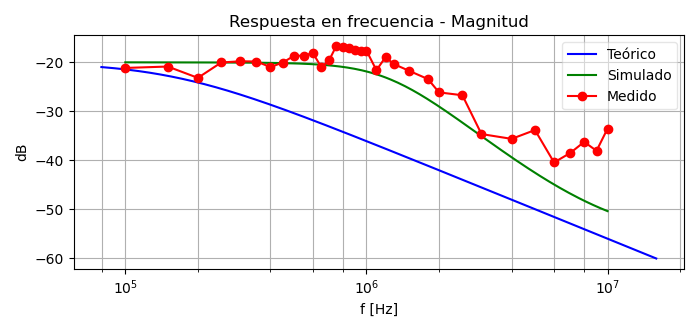
\includegraphics[width=.8\linewidth]{./Imagenes/InvCaso3Gain.png}  
		\caption{Inversor Caso 3. Respuesta en frecuencia teórica: ganancia}
	\label{fig:circinvcaso1}
\end{figure}

\begin{figure}[H]
	\centering
		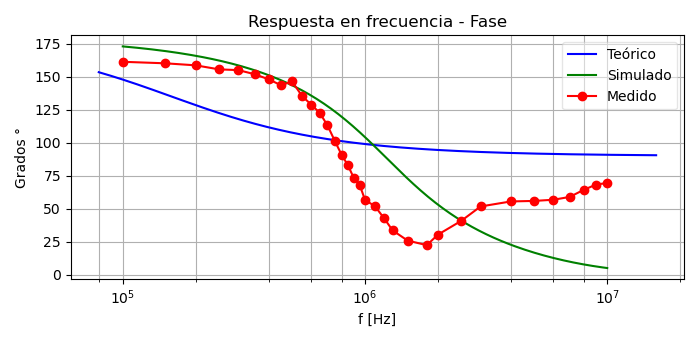
\includegraphics[width=.8\linewidth]{./Imagenes/InvCaso3Phase.png}  
		\caption{Inversor Caso 3. Respuesta en frecuencia teórica: fase}
	\label{fig:circinvcaso1}
\end{figure}


Aunque en distintos grados, se verifican diferencias y algunas coincidencias entre los casos teóricos, simulados y medidos. En general, se observa que las tres curvas coinciden a bajas frecuencias a un valor de la ganancia cercano al ideal y una diferencia de fase de $180^{\circ}$, verificando en ambos casos lo esperado por la teoría. 
Focalizando en los gráficos de ganancia, se observa una similitud entre el caso medido y el simulado, con los datos relevados directamente sobre el circuito acompañando bastante bien la curva simulada en el primer y segundo caso. 

En el tercer caso, en tanto, empieza a divergir a partir de una frecuencia del orden de los $10^{6} Hz$. Esto se puede deber a que para tomar las mediciones y evitar las limitaciones de SR vistas mas adelante, la señal de excitación fue de muy baja amplitud, dificultando las mediciones a frecuencias elevadas y haciendo susceptible de tomar una medición con ruido. Se decidió medir hasta una frecuencia de $10^{7} Hz$ para obtener un gráfico que se extienda una década por encima de la frecuencia de corte. Sin embargo, entendiendo las dificultades en la medición hubiera sido mejor limitar el rango de frecuencias para la medición.

Los gráficos de diferencia de fase muestran una desviación de los datos simulados y medidos respecto al modelo teórico de polo dominante, ya que continúan por debajo de los $90^{\circ}$. Esto último permite entender al circuito con el amplificador operacional como un filtro de segundo orden y no de primer orden como se había planteado en el modelo. Se verifica en el primer gráfico de la ganancia, por ejemplo, que la misma es atenuada en unos $-40dB$ en el rango de frecuencias de $10^{4} Hz$ y $10^{5} Hz$, es decir, una década. 

En el tercer caso, las diferencias entre la fase teórica, medida y simulada muestra las mayores diferencias. Primeramente los datos medidos arrojan un cambio mucho mas veloz en la diferencia de fase, pero a medida que aumenta la frecuencia los datos medidos se acercan al caso teórico. No es esperable éste comportamiento y es por ello que se tomaron las mediciones hasta tres veces intentando variar la disposición de los elementos en el circuito o los parámetros de la señal de entrada. Hay que tener en cuenta que debido a algunas características del circuito la señal de salida puede verse afectada y no mostrar la amplificación esperada. Se verán algunas limitaciones mas adelante. 

Concluyendo, considerando las mediciones del tercer caso como poco representativas por encima de los $10^{6} Hz$ debido a que pudieron a frecuencias por encima  haberse visto afectadas por distintos efectos del operacional o el circuito, se observa una similitud entre los casos medidos y simulados, que muestran el comportamiento del circuito como un filtro pasa bajo de segundo orden. 


\subsection{Circuito No Inversor}

\subsubsection{Análisis teórico}

Empleando las consideraciones vistas arriba y la relación \ref{eq:1}, se plantean las siguientes ecuaciones para el circuito no inversor de la Figura.:

Planteando un divisor resistivo para obtener la tensión en la entrada inversora del $OpAmp$:

$$v^{-}=\frac{R_{1}}{R_{1}+R_{2}}v_{out}$$

Y visualizando las siguientes relaciones:


\begin{equation} 
\left\{\begin{matrix}
	$v_{in}-R_{3}I_{3}=v^{+}$
	
	\\ 
	$I_{1}=I_{2}$
	
	\\ 
	
	$I_{3}=I_{4}=\frac{v^{+}}{R_{4}}$
	
\end{matrix}\right.
\end{equation}	
	

Reemplazando se llega a que la entrada no inversora del $OpAmp$ equivale a:

$$v^{+}=\frac{V_{in}}{1+\frac{R_{3}}{R_{4}}}$$

Reemplazando en la relación vista para la tensión de salida con las de entrada, se llega a la siguiente expresión:

$$\frac{v_{out}}{v_{in}}=\frac{A_{v_{ol}}(R_{1}+R_{2})R_{4}}{(R_{3}+R_{4})(R_{1}+R_{2}+R_{1}A_{v_{ol}})}$$

Asumiendo un modelo completamente ideal, para el cual la ganancia de tensión es infinita, se obtiene la ganancia del circuito equivale a lo siguiente: 

$$A_{v_{ol}}\underset{\infty }{\rightarrow} G_{ideal}=\frac{R_{1}R_{4}+R_{2}R_{4}}{R_{1}(R_{3}+R_{4})}$$

Considerando la ganancia de tensión como un valor constante, característico del amplificador:

$$A_{v_{ol}}=A_{ol}\Rightarrow \frac{v_{out}}{v_{in}}=\frac{A_{ol}(R_{1}+R_{2})R_{4}}{(R_{3}+R_{4})(R_{1}+R_{2}+R_{1}A_{ol})}$$

Con el modelo de polo dominante, obtenemos que la función transferencia resulta:

$$A_{v} = \frac{A_{ol}}{1+\frac{s}{w_{b}}}\Rightarrow H(s)=\frac{A_{ol}\frac{(R_{1}+R_{2})R_{4}}{q_{2}}}{\frac{s}{w_{b'}}+1}$$

\begin{equation}
\left\{\begin{matrix}
	$$q_{1}=(R_{3}+R_{4})(R_{1}+R_{2})$$
	
	\\ 
	$$q_{2}=(R_{3}+R_{4})(R_{1}+R_{2})+(R_{1}+R_{3})R_{1}A_{ol}$$
	
	\\ 
	
	$$w_{b'}=\frac{w_{b}q_{2}}{q_{1}}$$
	
\end{matrix}\right.
\end{equation}

Reemplazando los valores de los componentes especificados en la Tabla, se obtienen los siguientes valores de la ganancia y función transferencia para cada caso:

\begin{table}[H]
\centering
\begin{tabular}{c|c|c|c}
       & $A_{ol} = \infty$  & $A_{ol} = 10^{5}$ & $A_{v} = \frac{A_{ol}}{1+\frac{s}{w_{b}}}$ \\ \hline
Caso 1 & 8,6614  & $8,6604$  & $H(s)=\frac{8,66}{9,16\cdot 10^{-6}+1}$$  \\ \cline{1-1}
Caso 2 & 1,5748  & $1,5747$   & $H(s)=\frac{1,57}{1,66\cdot 10^{-6}+1}$  \\ \cline{1-1}
Caso 3 & 0,8661  & $0,8661$  & $H(s)=\frac{0,86}{0,916\cdot 10^{-6}+1}
\end{tabular}
\end{table}

\begin{figure}[H]
	\centering
	\begin{subfigure}{1\textwidth}
		\centering
		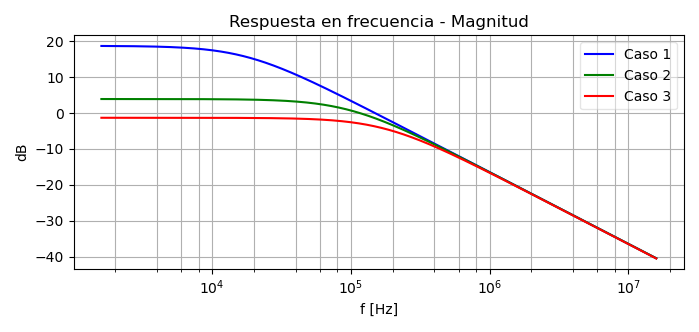
\includegraphics[width=.8\linewidth]{./Imagenes/NoInversorCasosGain.png}  
		\caption{Respuesta en frecuencia teórica: ganancia}
	\end{subfigure}
	\begin{subfigure}{1\textwidth}
		\centering
		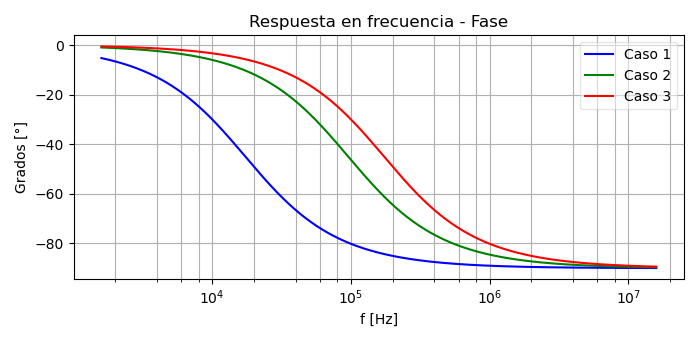
\includegraphics[width=.8\linewidth]{./Imagenes/NoInversorCasosPhase.png}  
		\caption{Respuesta en frecuencia teórica: fase}
	\end{subfigure}
	\caption{Circuito No inversor. Respuesta en frecuencia teórica.}
	\label{fig:Noinvcasos}
\end{figure} 

En la Figura \ref{fig:Noinvcasos} se visualizan las gráficas de las funciones transferencias correspondientes a los tres casos del circuito No inversor. Nuevamente, se observa que a bajas frecuencias 
las ganancias se corresponden con las mas ideales. Resulta interesante la expresión de la ganancia para esta configuración no inversora, 
debido a que se observa la participación de todos los resistores presentes en el circuito. También en esta configuración se observa que el Caso 1 es el de mayor ganancia y el Caso 3 el de menor. 

A medida que se incrementan las frecuencias, se ve el efecto del polo de primer orden incluido en el modelo, siendo especialmente notorio en el gráfico de la fase donde se llega
a una diferencia de hasta $90^{\circ}$ con la señal de entrada. Se observa que a altas frecuencias la ganancia en todos los casos es prácticamente la misma.

\subsubsection{Resultados}

A continuación se presentan los resultados obtenidos mediante mediciones y simulación, contrastados con la función transferencia teórica. Para la medici

\begin{figure}[H]
	\centering
	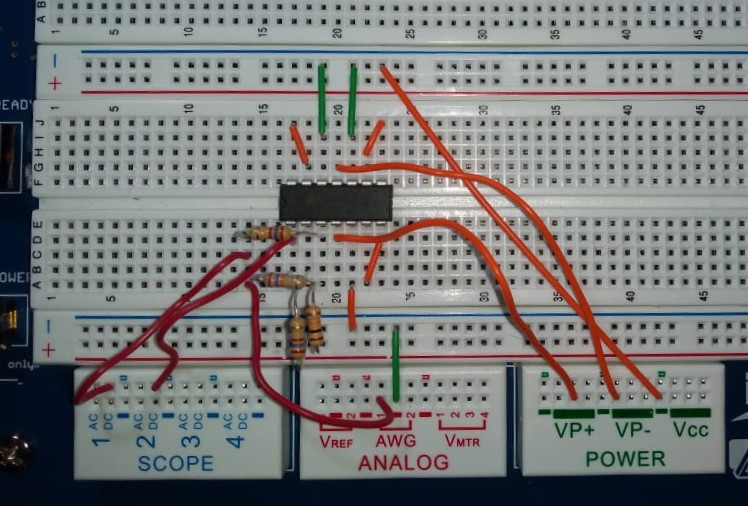
\includegraphics[scale=0.5]{./Imagenes/NoInv1Freq.jpeg}
	\caption{Circuito No inversor utilizado para las mediciones. Caso 1.}
	\label{fig:circnoinvcaso1}
\end{figure}

\begin{figure}[H]
	\centering
	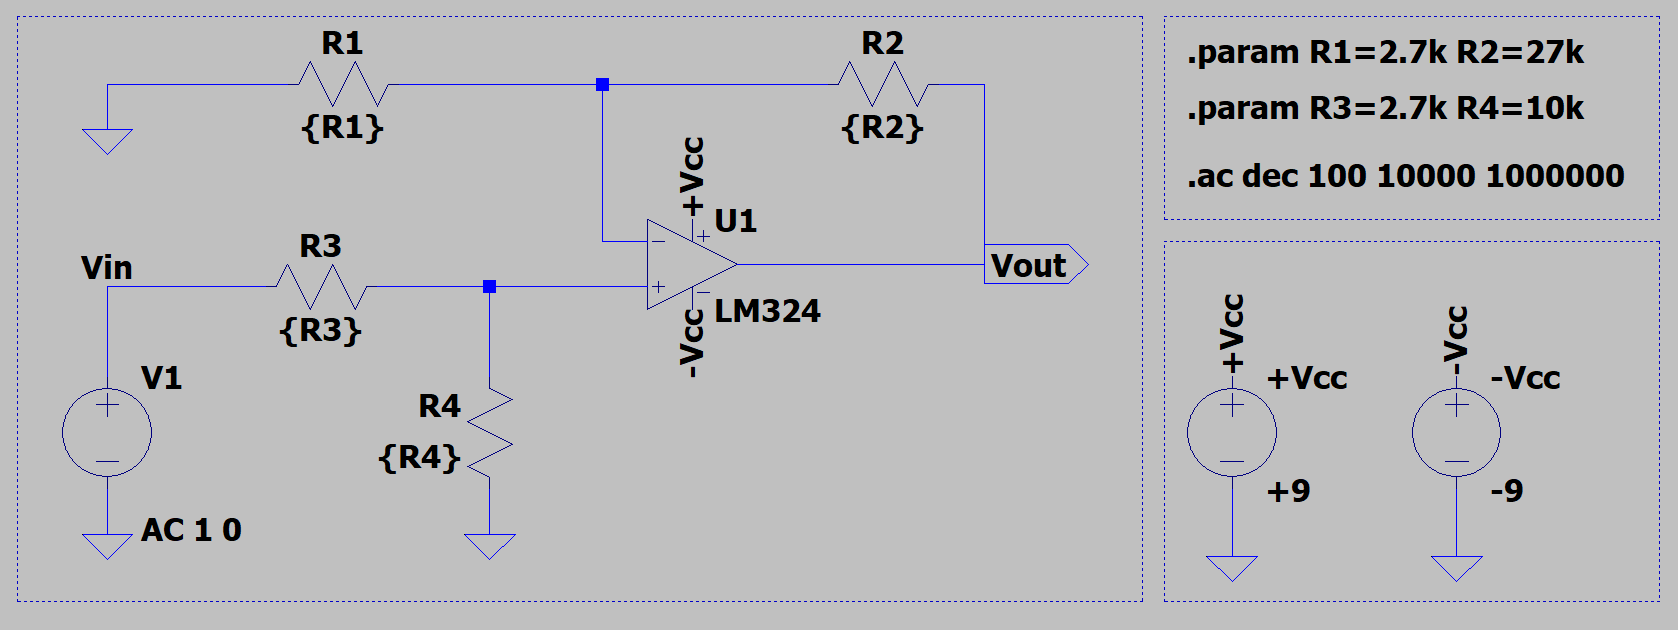
\includegraphics[scale=0.35]{./Imagenes/simuNoInv1.png}
	\caption{Esquema circuital no inversor Caso 1 en LTSpice.}
	\label{fig:circinvcaso1}
\end{figure}

Se superpusieron los resultados con la función transferencia teórica, obteniendo los siguientes resultados:

\begin{figure}[H]
	\centering
		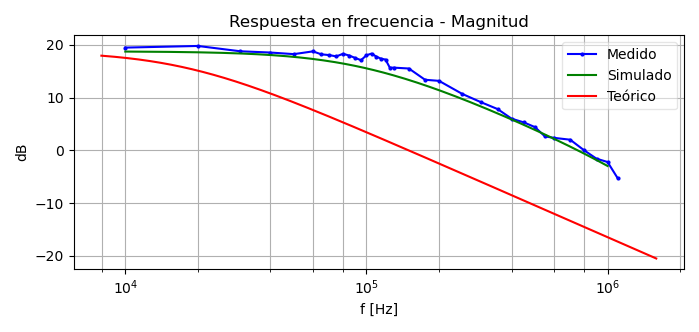
\includegraphics[width=.8\linewidth]{./Imagenes/NoInvCaso1Gain.png}  
		\caption{No inversor caso 1. Respuesta en frecuencia teórica: ganancia}
	\label{fig:circinvcaso1}
\end{figure}

\begin{figure}[H]
	\centering
		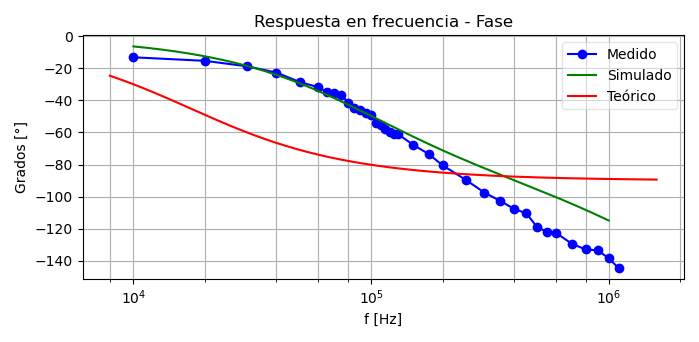
\includegraphics[width=.8\linewidth]{./Imagenes/NoInvCaso1Phase.png}  
		\caption{No inversor caso 1. Respuesta en frecuencia teórica: fase}
	\label{fig:circinvcaso1}
\end{figure}

\begin{figure}[H]
	\centering
		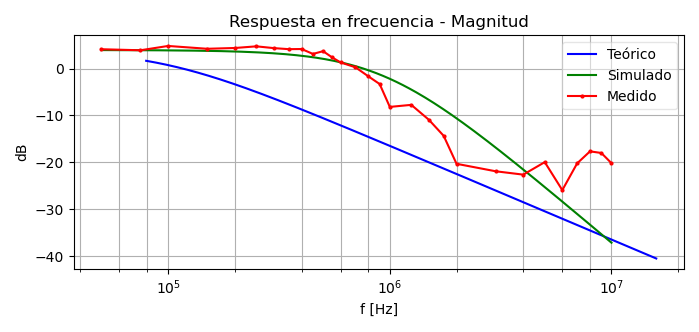
\includegraphics[width=.8\linewidth]{./Imagenes/NoInvCaso2Gain.png}  
		\caption{No inversor caso 2. Respuesta en frecuencia teórica: ganancia}
	\label{fig:circinvcaso1}
\end{figure}

\begin{figure}[H]
	\centering
		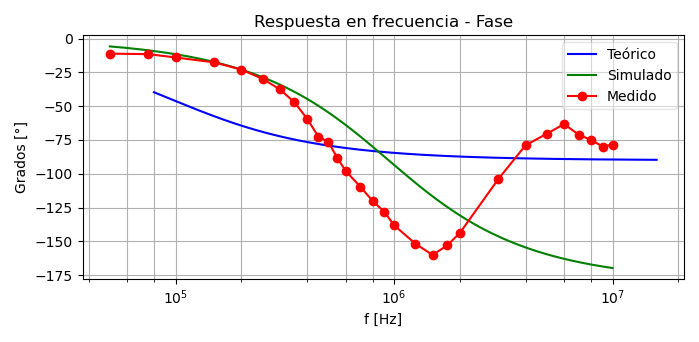
\includegraphics[width=.8\linewidth]{./Imagenes/NoInvCaso2Phase.png}  
		\caption{No inversor caso 2. Respuesta en frecuencia teórica: fase}
	\label{fig:circinvcaso1}
\end{figure}

\begin{figure}[H]
	\centering
		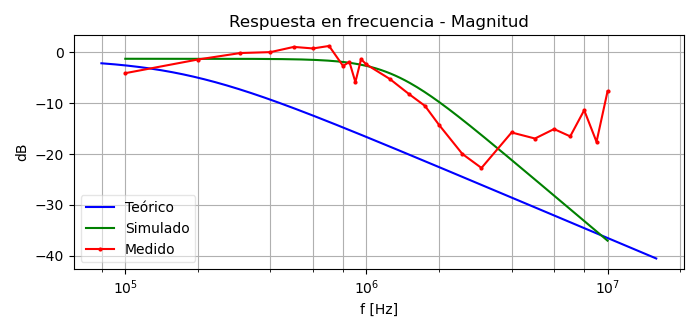
\includegraphics[width=.8\linewidth]{./Imagenes/NoInvCaso3Gain.png}  
		\caption{No inversor caso 3. Respuesta en frecuencia teórica: ganancia}
	\label{fig:circinvcaso1}
\end{figure}

\begin{figure}[H]
	\centering
		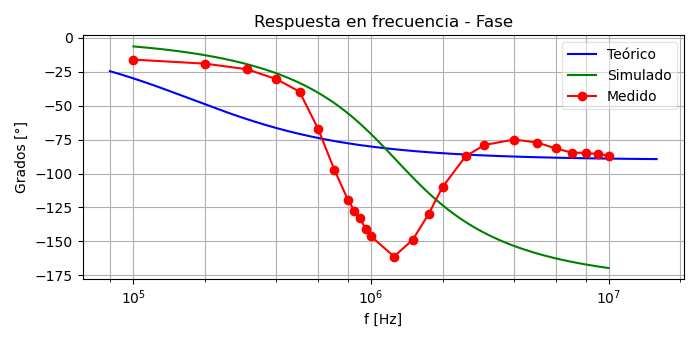
\includegraphics[width=.8\linewidth]{./Imagenes/NoInvCaso3Phase.png}  
		\caption{No inversor caso 3. Respuesta en frecuencia teórica: fase}
	\label{fig:circinvcaso1}
\end{figure}

Aunque a bajas frecuencias tienden a mostrar valores similares a los de las ganancias ideales, en los tres casos se observan discrepancias entre los valores del modelo teórico, simulado y de las mediciones. Por los datos relevados de la simulación, se visualiza que el amplificador muestra una respuesta correspondiente a un filtro pasa bajo de segundo orden. Sin embargo, los datos medidos no acompañan ese comportamiento. 
De hecho, único caso en el que los resultados entre los valores simulados y medidos se asemejan es en el primer caso, en el cual la gráfica permite observar incluso una atenuación menor de la ganancia con la frecuencia respecto a lo predicho por la función transferencia. 

En los casos 2 y 3, si bien hasta altas frecuencias no presentan grandes diferencias, a medida que se acerca a frecuencias del orden de los $10^{7} Hz$ los datos medidos arrojan inconsistencias, ya que muestra un incremento notable en la ganancia. De la misma forma que se describió en los resultados del circuito inversor, esto se puede deber a que para frecuencias por encima de los $10^{6} Hz$ las señales de salida están muy atenuadas (hay que considerar que son los dos casos de menor ganancia) y se introduce mucho ruido en la medición. 

Tomando en cuenta las características del circuito y del operacional (vistas en próximas secciones), para realizar las mediciones se estimuló el circuito con señales senoidales de baja amplitud (entre 150 y 300 $V_¨{pp}$, dependiendo del circuito). Esto, contando con la pobre ganancia en los casos 2 y 3, pudo haber afectado las mediciones a altas frecuencias, llegando a las incongruencias con los valores esperados por los demás modelos. Primeramente, ante la falta de coherencia de los valores registrados, se realizaron algunas mediciones hasta tres veces intentando cambiar la disposición circuital o algunos parámetros, pero en ningún caso se logró conseguir valores mas cercanos a los esperados. Se concluye para futuras mediciones limitar el rango de frecuencias utilizadas para la medición cuando se empleen circuitos de baja ganancia.   

Donde se encuentran mayores disimilitudes son en los gráficos de la diferencia de fase. No obstante, aprovechando que el gráfico del primer caso muestra los valores mas limpios de los tres, se puede observar con claridad que el amplificador operacional actúa como un filtro pasa altos de segundo orden dado que la diferencia de fase sigue por debajo de los $90^{circ}$. En cuanto a los demás casos, se observa ese comportamiento hasta los $10^{6} Hz$; para frecuencias mas altas, se visualizan comportamientos que se apartan de lo esperado. 






